\documentclass[a4paper,11pt, oneside]{book}
\usepackage[utf8]{inputenc}
\usepackage[english]{babel}
\usepackage[T1]{fontenc}
\usepackage{graphicx}
\usepackage{float}
\usepackage{wrapfig}
\usepackage{setspace}
\usepackage{geometry}
\usepackage[hidelinks]{hyperref}
\usepackage{multicol}
\usepackage{etoolbox}
\usepackage{color}
\usepackage[explicit,pagestyles]{titlesec}
\usepackage[absolute,overlay]{textpos}
\usepackage{fancyhdr}
\usepackage{fontspec}
\usepackage{eurosym}
\usepackage{titlesec}
\usepackage[]{algorithm2e}


% ====== CONFIG ========

\graphicspath{{img/}}
\setlength{\unitlength}{1mm}
\makeatletter

\definecolor{primary}{RGB}{44, 62, 80}


\titleformat{\chapter}[display]{\huge}{\thechapter \quad #1}{0pt}{}
\titlespacing{\chapter}{0pt}{0pt}{0pt}

\titleformat{\section}[display]{\LARGE}{}{0pt}{\thesection \quad #1}


\setlength{\TPHorizModule}{1mm}
\setlength{\TPVertModule}{1mm}
\def\sizeMedia{38}
\def\size{3.8cm}
\def\sizeMargin{0.2cm}
\def\margin{2}
\def\fixMargin{0}

\pagestyle{plain}

\author{Luc Dupuis, Quentin Tardivon, Ragul Sankar, Asmita Belle}
\date{\today}

\def\school{Maynooth University}
\def\schoolAddress{Maynooth, Co. Kildare}
\def\schoolYear{2017}

\def\appName{Hackoeur Android}
\def\widthImage{1}
\def\todo{{\color{red}\Huge{TODO}}}

% ====== END CONFIG ========


\begin{document}

	\begin{titlepage}
		\thispagestyle{empty}

{\color{primary}

\hspace{4.5cm}

\includegraphics[width=6.0cm]{img/maynooth.png}



\vspace{0.5cm}

	\begin{center}


			{\color[rgb]{0.8,0.8,.8}\rule{\textwidth}{0.8pt}}
			\vspace{0.5cm}

			\baselineskip=3pt
			{\Huge \bfseries{\appName}}\\
			\vspace{0.2cm}
			{\huge \bfseries{CS385: Android Development}}
			\vspace{0.5cm}

		{\color[rgb]{0.8,0.8,.8}\rule{\textwidth}{0.8pt}}
		\vspace{0.5cm}


		
\includegraphics[width=10cm]{logo.png}

		\vspace{4cm}
		\Large{Luc Dupuis}\\
		\Large{Quentin Tardivon}\\
		\Large{Ragul Sankar}\\
		\Large{Asmita Belle}

		\vspace{0.5cm}
		\large{\schoolYear}
	\end{center}

}

	\end{titlepage}


	\newpage\newpage\null\thispagestyle{empty}
	\newpage
		\tableofcontents
		\thispagestyle{empty}


	\chapter{Introduction}
	\setcounter{page}{1}

	This document is presenting technical details of the CS385 Android Development
	Project. This project is called Hackoeur and is an application to create Tech related events and
	Hackathons. It has been realized by Luc Dupuis, Quentin Tardivon, Ragul Sankar and Asmita Belle.
	In a first part we will describe how to use the application and in the second part we will discuss
	technical choices for each activity.

	\chapter{How to Use}

	In order to use Hackoeur, you need to have at least Android 6.0 (note that the application has been
	mainly tested on Android 8.0) and an available Google Account. When you are opening the application for
	the first, you have to log in with your Google Account. After that, you will always be automatically
	connected with this account. If you want to change account, you can disconnect in the top-left menu.

	The app is organized in 3 main fragments all regrouped in the same MainActivity. The first tab represent
	all the available created events, the second one the list of every registered users and finally a list 
	and a map representing your saved events. You can click on a event at every moment to display details of
	the event and have access to the button allowing you to save the event. 

	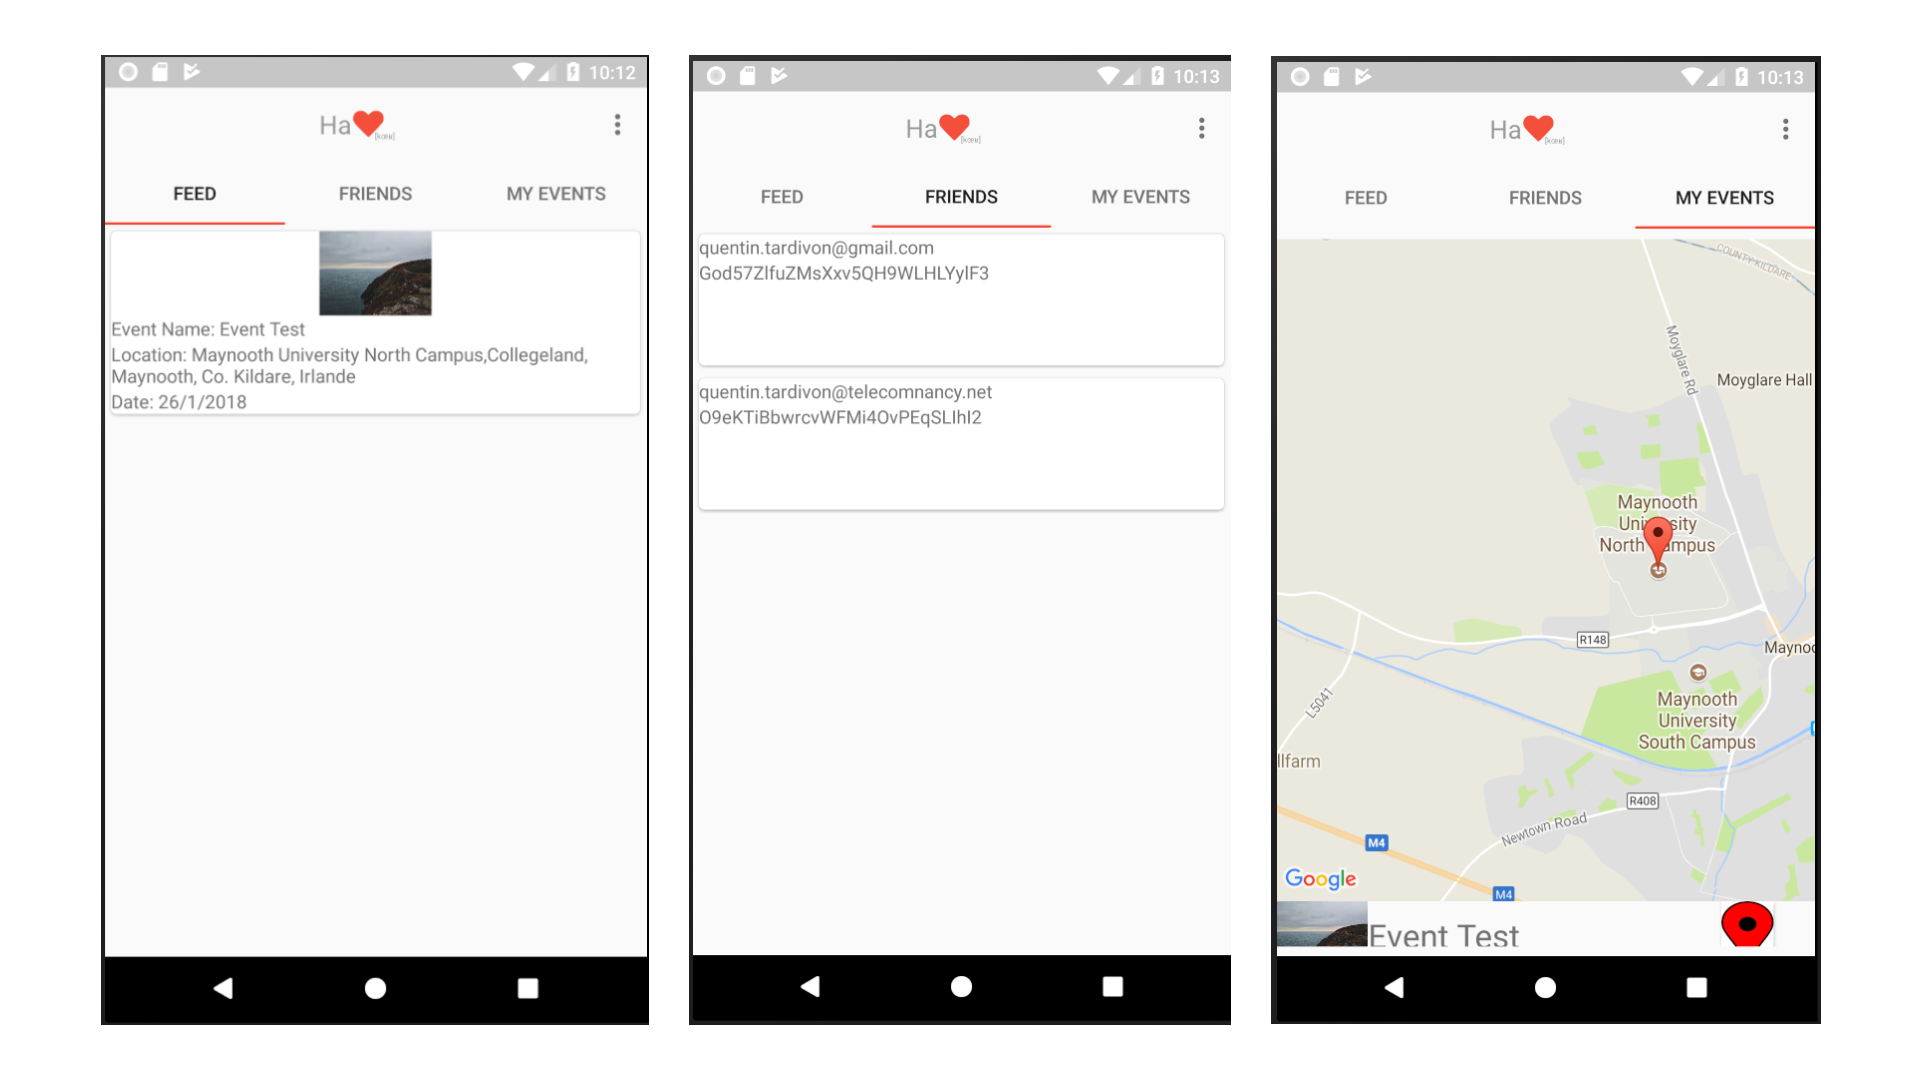
\includegraphics[width=13cm]{./img/views.png}

	If you want to create an event, you have access to the creation page from the top-left menu.
	Once you are on the creation page, you have to type a name, a description, use the map tool for a location, 
	a date and upload an image for your event. After your image is successfully uploaded, you can click on 
	the create button and your event will be displayed in the event list. If you are creating an event, it is
	automatically added to your saved events. You can't delete an event or modify it at the moment, so be careful when you create your event. 
	
	\chapter{Implementation}

	For this project, we are using the latest technology available for Android: Backend with Firebase, Kotlin Programming 
	Language and Adaptable Icon. The whole project is hosted on Github and is completely open-source. We used github 
	during the whole project as hosting service but also as collaborative tools which allowed us to work asynchronously on
	the same project, each team member with these own API keys. If you want to build the project, it is necessary to obtain
	API keys for Firebase and Google Maps and to follow the instruction to configure these services in Android Studio project. 


		\section{Splash Screen}

		When you are opening the application, the first thing that is displayed is the SplashScreen.
		We use the splashscreen to initialize our Firebase Services that are responsible for
		login operations, store events and store event pictures. We are respectively using
		Firebase Authentication, Firebase Database and Firebase Storage for these actions.
		As soon as the services are loaded we are launching the Main Activity.

		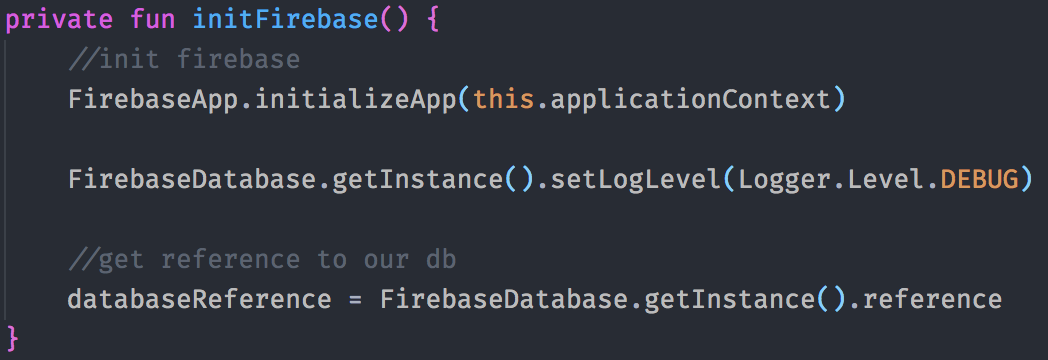
\includegraphics[width=13cm]{./img/initfire.png}

		\section{Login Page}
		
		At the first app launch, the MainActivity is launching the Login Screen and ask the user 
		to Log In with a Google Account. If the user does not have a Google Account, there is a button 
		which open a Web Page to create a Google Account. We are using Firebase Authentication with Google Sign-In
		to simplify the whole process: we don't have to store any credentials and the user does not have a specific account
		for the application.

		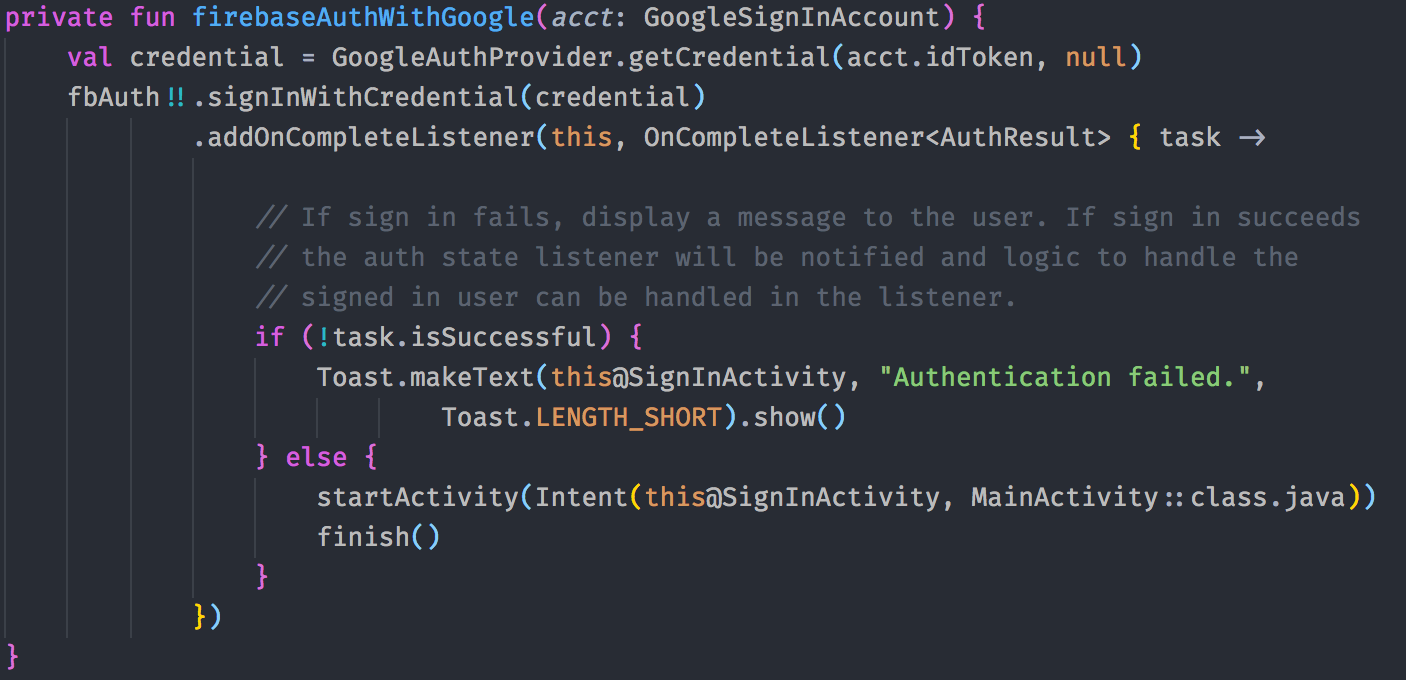
\includegraphics[width=13cm]{./img/firebaseauth.png}

	\section{Main Activity}

	The Main Activity is based on a TabLayout with 3 differents tab: 
	\begin{itemize}
		\item Event List
		\item Friends List
		\item My Events
	\end{itemize}
		In order to use this system, we implemented a TabPager Adapter which display different Fragments based on 
		what tab is currently selected.
		
		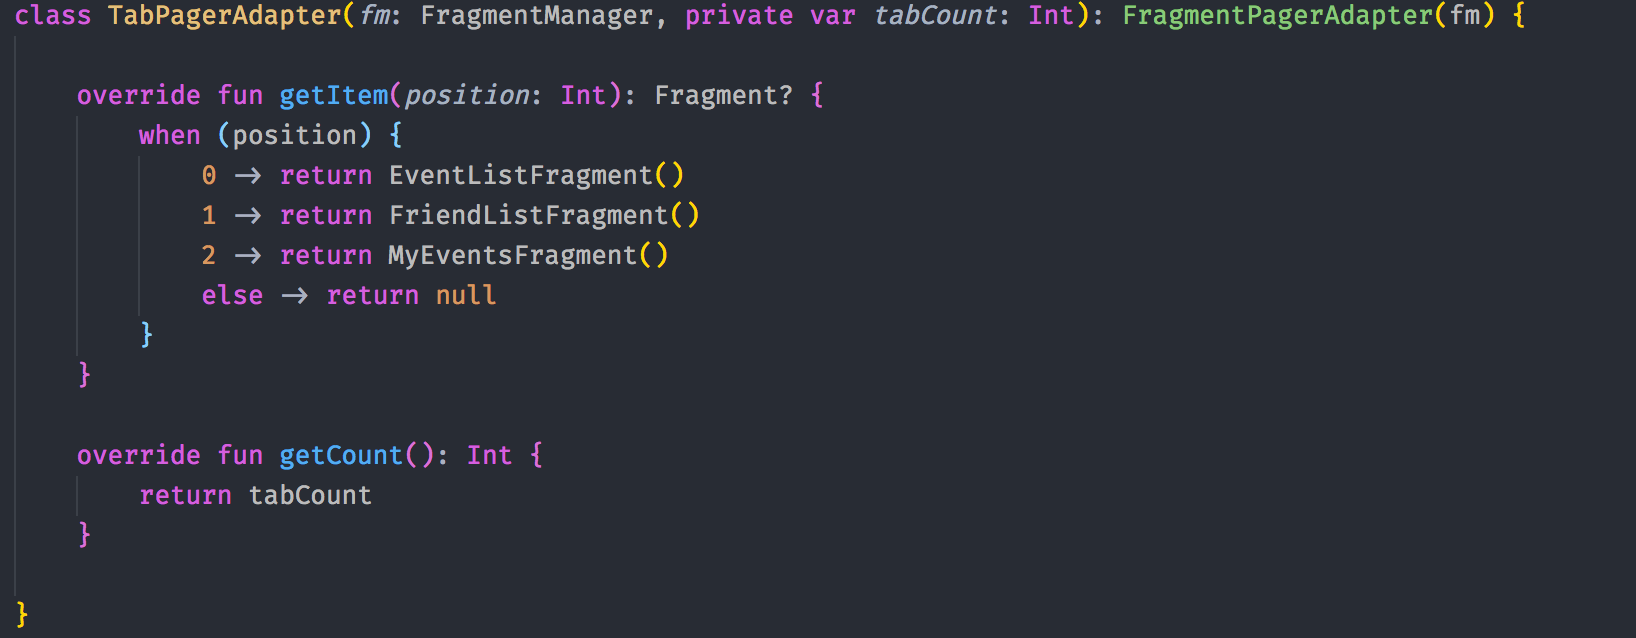
\includegraphics[width=13cm]{./img/tabpager.png}

		\subsection{Event List}	

		The Event List is using 3 main elements: 
		\begin{itemize}
			\item Event
			\item EventAdapter
			\item EventListFragment
		\end{itemize}

		We created a Event class containing all the information for an Event. We created a EventAdapter allowing
		us to display all the event from the Firebase Database and we finally used the EventListFragment to display this 
		adapter. Since we are using the Firebase Database, we are listening asynchronously to the push event in the database, 
		thus if a user create an event it is automatically added and display to all the user without app refreshing.

		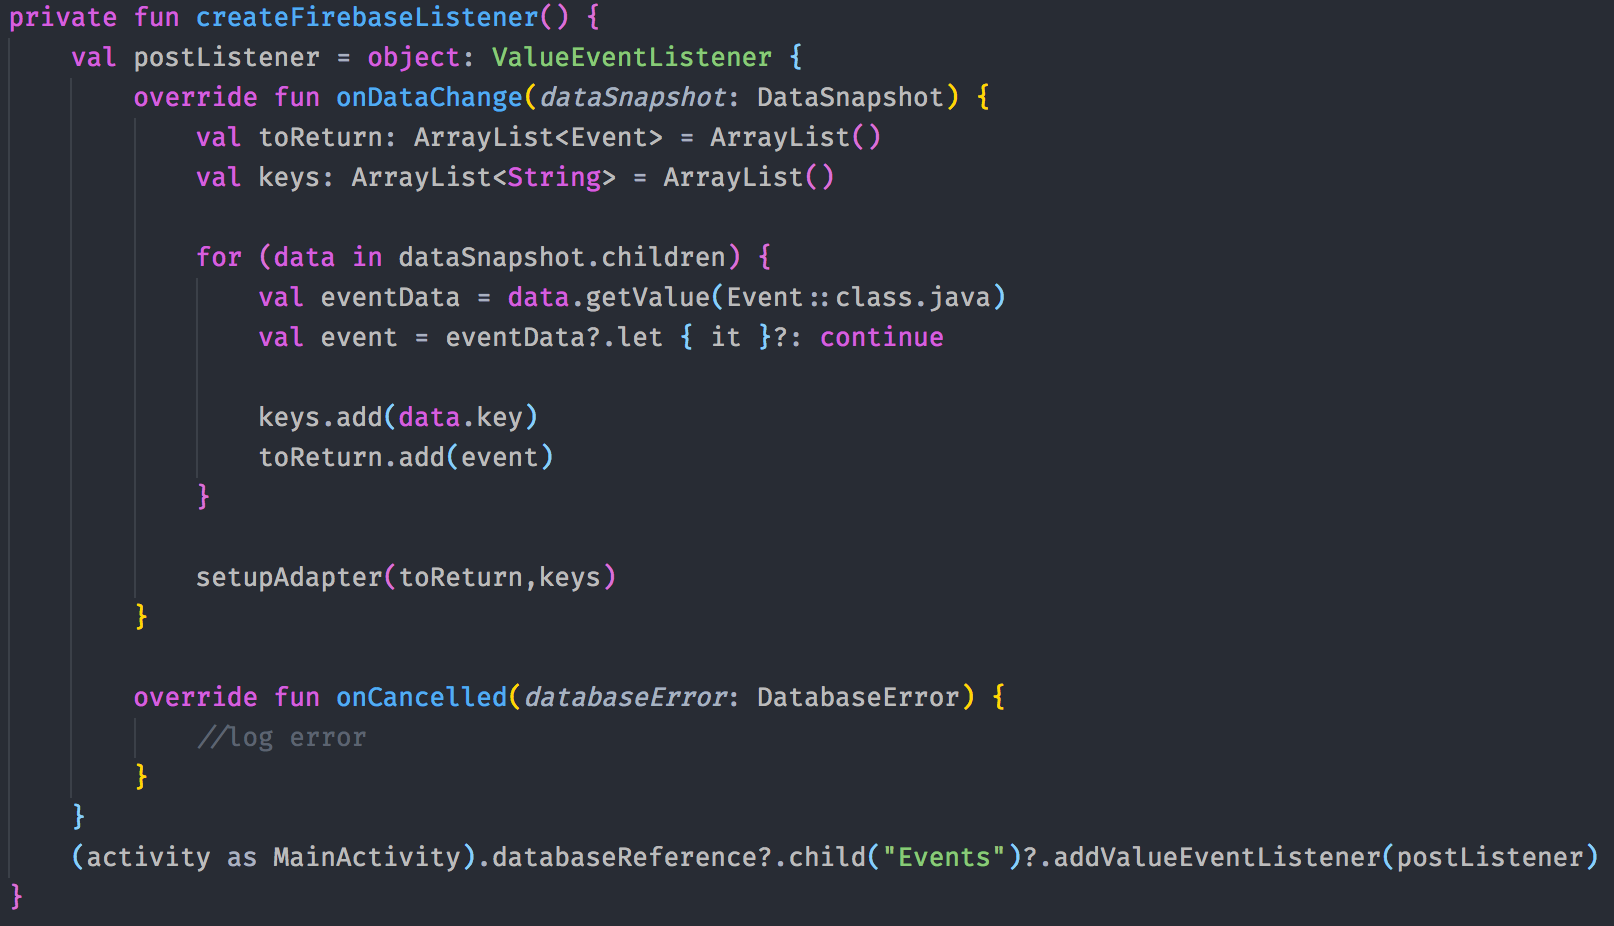
\includegraphics[width=13cm]{./img/firebaselistener.png}

		We also had to implement the Event object as Parcelable in order to pass it from an activity to another with the Intent
		system. Indeed since its a complex object and not a simple String or Int, we have to describe how the object is created
		and in which order each argument are coming to be able to reconstruct the object in the activity receiving the Intent.

		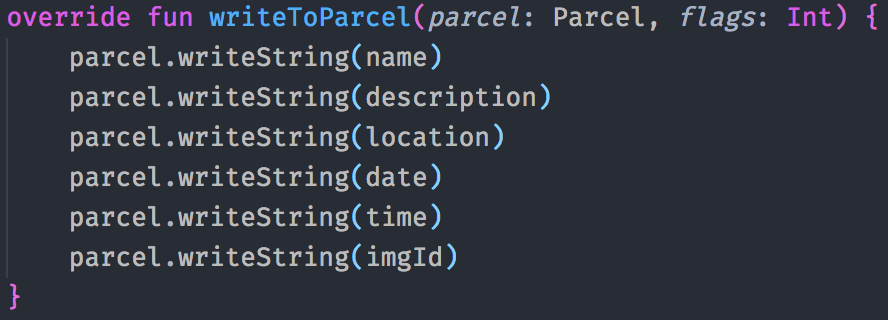
\includegraphics[width=13cm]{./img/parcelable.png}

		\subsection{Friend List}

		The Friend list is using exactly the same structure as Events:
		\begin{itemize}
			\item User 
			\item UserAdapter
			\item FriendListFragment
		\end{itemize}

		The user is added to the database at its first login. After that, each user have a unique key which allow us to identify
		them.

		\subsection{My Events}

		The saved event list is a bit different because it add a Google Map which allow us to see the location of the events. Its
		using a different adapter but is follwing the principles as the main EventList. We had to create a LatLng object which store
		the coordinates of an events to display them on the map.

		\section{Create Event}

		\section{Event Description}

	\chapter{Possible improvements}

	There is still a lot of possible improvements. The first thing would be to fix the performance issues introduce
	with images on events. We can add the possibility to modify and delete created events. We can also add informations about
	users and a user page. We can add the possibility to see which events are saved by users.

	\chapter{Conclusion}

	We learnt a lot during this project about the development cycle of an Android App. We had the opportunity to use the latest
	tools for Android development. We saw how to use Parcelable, TabPager, Google Maps API, Firebase tools and Kotlin languages.

\end{document}
